% ---------------------------------------------------------------------------
% Insert in \subsection{Born-Oppenheimer formalism and the eikonal approximation},
% directly after the sentence
%   "Observables must not depend on $\vee$, since changing it only moves modes
%    between the two sectors."
% (needs \usepackage{graphicx}; rapidity_layout.pdf next to the main file)
% ---------------------------------------------------------------------------
The longitudinal layout of the calculation is summarised in Fig.~\ref{fig:rapidity}.
The valence modes, $k^{+}\geq\vee$, enter only through their colour-charge density
$\rho^{a}(\mathbf{x})$. The soft window $\Lambda<k^{+}<\vee$ spans the rapidity interval
$\delta Y=\ln(\vee/\Lambda)$, and the soft gluon cloud of the projectile is built inside it. The target
moves in the $-$ direction with large $P^{-}$. In the frame used here its field $A^{-}$ is
localised at $x^{+}\simeq0$ and acts on the projectile as a shock wave, through the adjoint Wilson
lines $U(\mathbf{x})$ of the eikonal $S$-matrix (Sec.~\ref{sec:production}). Modes with $k^{+}<\Lambda$
are not part of the projectile wave function; they belong to the target. A gluon measured at
mid rapidity, $\vee\gg k^{+}\gg\Lambda$, splits the soft window in two. Soft gluons harder than the
measured one, $k^{+}<p^{+}<\vee$, act as additional colour sources of the projectile and generate the
$\ln(\vee/k^{+})$ term: the BFKL evolution of the projectile (KLWMIJ for a dense projectile).
Softer gluons, $\Lambda<p^{+}<k^{+}$, resolve the target and generate the $\ln(k^{+}/\Lambda)$ term,
the JIMWLK evolution of the target. The two logarithms add up to $\delta Y$. The dependence on
$\vee$ and $\Lambda$ is thus absorbed into the evolution of the projectile and of the target,
respectively, and the remaining terms are finite as $\Lambda\to0$ and $\vee\to\infty$.

\begin{figure}[t]
  \centering
  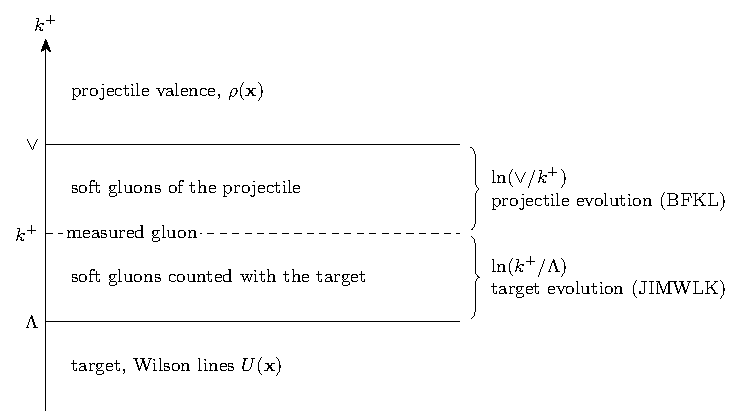
\includegraphics[width=0.75\textwidth]{rapidity_layout.pdf}
  \caption{Partition of the longitudinal momentum $k^{+}$. Valence modes ($k^{+}>\vee$) act through
  $\rho^{a}(\mathbf{x})$; the soft window $\Lambda<k^{+}<\vee$ has width $\delta Y=\ln(\vee/\Lambda)$. The
  measured gluon at $k^{+}$ splits the window: soft gluons above it belong to the projectile and give
  $\ln(\vee/k^{+})$ (BFKL), those below it are counted with the target and give $\ln(k^{+}/\Lambda)$
  (JIMWLK). The target ($k^{+}<\Lambda$) enters only through the Wilson lines $U(\mathbf{x})$.}
  \label{fig:rapidity}
\end{figure}
